\documentclass[10pt,a4paper]{article} 
\usepackage{graphicx}
\usepackage{caption}

% define the title, author and date of this document:

\title{Implementation of Succinct Dynamic Dictionary}
\author{Pablo Estrada @ Seoul National University}
\date{Dec. 2014}

% the printed part of the document starts here:

\begin{document}

% first print out the title:

\maketitle

% our article is divided into sections and subsections like this:

\section{Introduction}

This project set out to implement the succinct dynamic dictionary 
data structure presented in \cite{ramansatti2003} using C++. The paper also
specifies an Extendible Array structure that was implemented. We
will describe how these structures were implemented, as well as the
organization of the code, results, conclusions and future work.

\section{Structure of the code}

The project was implemented in C++. The code structure of the project contains 
directories \verb|src/|, \verb|include/|, and \verb|test/|. These directories 
contain, respectively, the code implementation of the structures, the
 include headers of the structures, and the test files implemented during the
 development of the project.

The data structures defined in the paper were the extendible array, which was implemented
 by the \verb|ExtendibleArray| class, which was fully implemented in the files 
\verb|extendible_array.h| and \verb|extendible_array.cc|; and the succinct 
dynamic dictionary, which was implemented by the \verb|SuccDynamicDict| class, 
in the \texttt{succinct\_dynamic\_dict.h} and \texttt{succinct\_dynamic\_dict.cc} files.

Particularly, the succinct dynamic dictionary requires the use of many elements,
and therefore, it utilizes some classes that provide functionality to it. Namely,
the \verb|LittleHash| class, the \verb|DynamicPerfectHash| class, and the 
\verb|ExtendibleArray| class. The \verb|LittleHash| class is in the
\texttt{little\_hash.cc} file, and its headers are in the \verb|little_hash.h| file;
while the \texttt{DynamicPerfectHash} class is implemented in the 
\texttt{dynamic\_perfect\_hash.cc} file, and its headers are in the 
\texttt{dynamic\_perfect\_hash.h} file. The functions and headers that are required by
all the elements of the project are contained in the \texttt{advanced\_arrays.h} file.

Finally, the \verb|test/| directory contains all the testing developed for this project.
The project is designed to be as general as possible; but the testing was done only with
\verb|int| and \verb|long int| element types. To run the full test suite, just run the
\verb|run_tests.py| script in the test directory.

\subsection{The \texttt{ExtendibleArray} class}

The \verb|ExtendibleArray| class is implemented similarly to the one suggested in
\cite{brodnik99}. It consists of a single index block that holds pointers to \emph{N}
data blocks of sizes \emph{1, 2,...,N}. In this structure, the first \(k\) blocks can
hold up to \(k(k+1)/2\) elements; and we can support access in \(O(1)\) time; as well
as grow and shrink operations in \(O(1)\) amortized time, with at most \(O(\sqrt{k})\)
extra memory used.

\begin{figure}[h!]
  \centering
\captionsetup{justification=centering}
  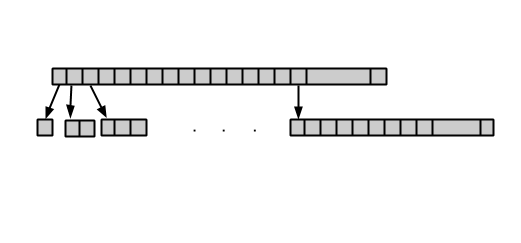
\includegraphics[width=0.5\textwidth]{ea_figure}
\caption{\emph{The form of the ExtendibleArray class. \\*Observe the index array at the top,
and the smaller arrays\\* that are pointed to by it.}}
\end{figure}

\subsection{The \texttt{LittleHash} class}
The \texttt{LittleHash} class is a self-contained small hash table that is able to
rehash and resize itself if necessary. It provides full dictionary functionality to the
\texttt{DynamicPerfectHash} class, which uses many instances of the \texttt{LittleHash}
to implement a dynamic perfect hashing algorithm. The underlying array is implemented
using an \texttt{ExtendibleArray} instance. It provides \(O(1)\) time membership query, and 
removal; as well as expected \(O(1)\) insertion time.

\subsection{The \texttt{DynamicPerfectHash} class}
The \texttt{DynamicPerfectHash} class implements dynamic perfect hashing as explained
by Dietzfelbinger \textit{et al.} in \cite{DM1994}. This class provides dictionary
functionality to the \texttt{SuccDynamicDict} class. It gives guaranteed worst-case 
constant time membership query and removal; as well as expected \(O(1)\) insertion
in efficient space.

\subsection{The \texttt{SuccDynamicDict} class}
The \texttt{SuccDynamicDict} class is the main goal of the project. It is the 
implementation of a succinct dynamic dictionary as explained by Raman and Satti 
in \cite{ramansatti2003}. It provides succinct dictionary functionality by constructing
a constant-height tree that uses the most significant bits to hash elements, and
compress away those bits.

\section {Results}

\subsection{Memory savings of \texttt{ExtendibleArray} class}
The \texttt{ExtendibleArray} class provides significant memory savings as compared 
to available extendible array implementations. Figure~\ref{mem_usage_4k4k} shows the
memory usage of the \texttt{ExtendibleArray} class when inserting and then removing
4 thousand elements; as opposed to the standard \texttt{Vector} class available for C++.
As shown by figure ~\ref{mem_usage_4k4k}, our extendible array shows less memory usage most of the time,
and only marginally higher for short periods. 

Another way of looking at this advantage is shown in figure~\ref{extra_mem_per_n}, 
where the ratio of extra memory usage over number of elements is plotted. As we can see,
since our extendible array grows in smaller increments, the impact on the memory is not
as dramatic. It should be observed that the advantage of the \texttt{ExtendibleArray} 
class does not show until after about 12 elements; where the extra cost of keeping an
index block is overshadowed by the allocation of \(O(n)\) extra space by the common
implementations of extendible arrays.

A disadvantage of the \texttt{ExtendibleArray} class is that although its access time is
\(O(1)\) asymptotically; in machine operations, the two memory accesses and memory operations
are evidently slower than a normal extendible array implementation that requires only a 
simple addition and memory access.

\begin{figure}[h!]
\captionsetup{justification=centering}
  \centering
\centering
  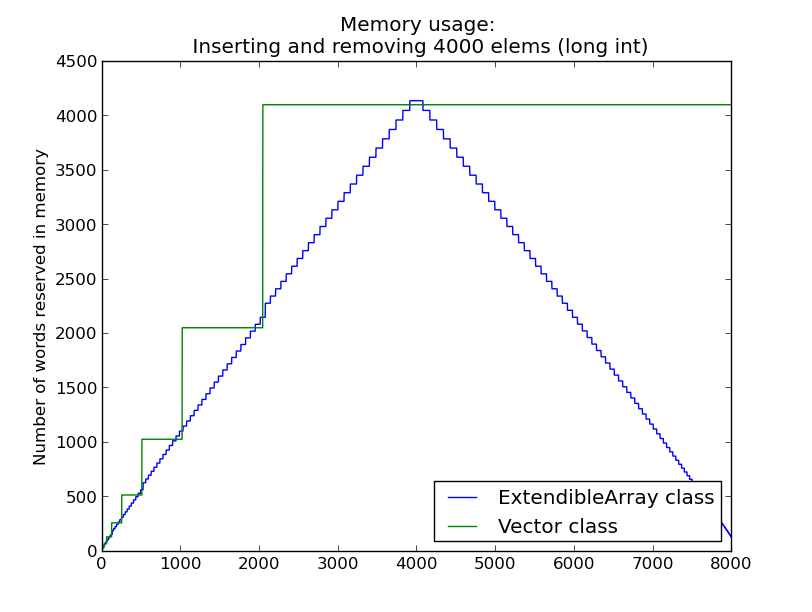
\includegraphics[width=0.5\textwidth]{mem_usage_4k4k}
\caption{\emph{The memory usage of both classes after inserting and removing 4,000 elemets}}
\label{mem_usage_4k4k}
\centering
  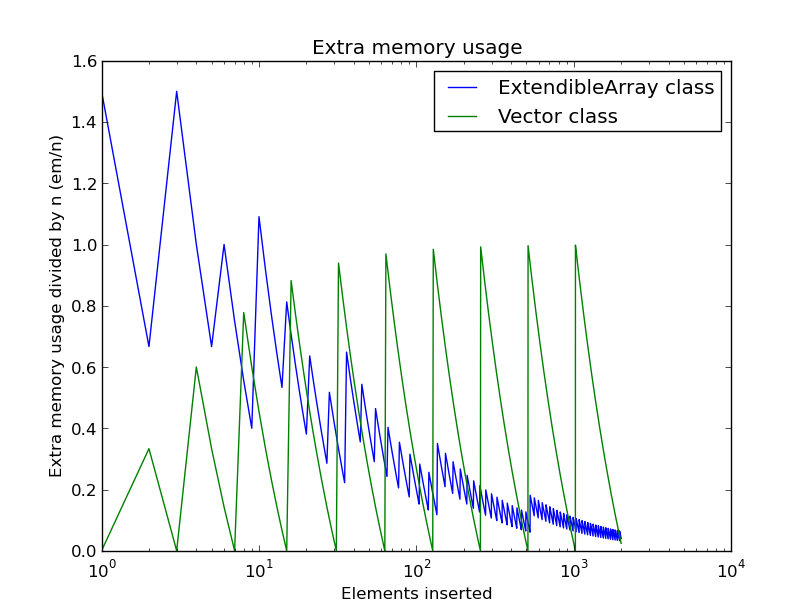
\includegraphics[width=0.5\textwidth]{extra_mem_over_n_log}
\caption{\emph{The memory usage of the \texttt{ExtendibleArray} class.}}
\label{extra_mem_per_n}
\end{figure}

\subsection{The dictionary classes}
The \texttt{DynamicPerfectHash} class provides efficient dictionary functionality.
Tests so far have shown good insertion and lookup performance, without any apparent
memory leak after rehashing or reshuffling.

The implementation of the \texttt{SuccDynamicDict} class has not been concluded as of 
Dec 4th of 2014. For now, we have opted to keep 64-bit length structures for each of the
recursive levels of the succinct dynamic dictionary. This eliminates any memory savings
that could be achieved from a normal non-succinct tree implementation. 
The main challenges for full implementation are the use of data structures that support 
per-byte operations, and packing of information in different-than-word-size memory
structures.

\section{Future work}
After finishing the implementation of the \texttt{SuccinctDynamicDict} class, we will focus
on tight packing of the memory structures to push memory usage down to the
theoretical limit in \cite{ramansatti2003}.

Also, immediately after that, we will work on benchmarks and tests to
 compare the memory usage of our dictionary classes as opposed to other
 implementations of similar structures both in the academic community and in 
publicly available software APIs. Another important measure is the access
time of the \texttt{ExtendibleArray} class as opposed to the C++ \texttt{Vector}
class.

\section{Conclusions}
We have implemented a set of classes that provide extendible array functionality in 
efficient space, as well as dictionary functionality. They present some advantages
such as generally lower memory usage and extra memory usage. Unfortunatelly, as of
now, there is not enough data and testing to evaluate the dictionary classes as
opposed to other similar implementations.

All the tests and code are available on \texttt{github.com/pabloem/advanced\_arrays}.

\begin{thebibliography}{9}
\bibitem{ramansatti2003} Rajeev Raman and S.Srinivasa Rao,
  \emph{Succinct Dynamic Dictionaries and Trees}.
  Automata, Languages and Programming. 
  Springer Berlin Heidelberg, 2003. 357-368.

\bibitem{brodnik99} A.Brodnik, S.Carlsson, E.D.Demaine, J.I. Munro and R.Sedgewick.
  \emph{Resizable arrays in optimal time and space}. 
  In \emph{Proc WADS '99}, LNCS 1663, 37-48.

\bibitem{DM1994} Dietzfelbinger, Martin, \textit{et al.}
  \emph{Dynamic perfect hashing: Upper and lower bounds}.
  SIAM Journal on Computing 23.4, 1994: 738-761.

\end{thebibliography}

\end{document}

